%%%%%%%%%%%%%%%%%%%%%%%%%%%%%%%%%%%%%%%%%%%%%%%%%%%%%%%%%%%%%%%%%%%%%%%%
\chapter{Process Manager/Thread Scheduler}
\label{sec:process_manager}
%%%%%%%%%%%%%%%%%%%%%%%%%%%%%%%%%%%%%%%%%%%%%%%%%%%%%%%%%%%%%%%%%%%%%%%%

MacSim uses a common Process Manager/Thread Scheduler for both CPU threads and
GPU warps. For each application that is to be simulated, the Process Manager
creates a process and also creates the threads/warps in the application. Based
on the simulation configuration, the Process Manager assigns cores to each
application, these cores are dedicated to the application. In case of CPU
applications, only the main thread of the application is launched first. The
trace configuration that is an input to the simulator specifies in terms of instructions
executed by the main thread when each child thread should be started. When a
child thread becomes ready for execution, the Process Manager is responsible
for assigning the child threads to cores. In case of GPU applications, the
Process Manager creates warps and forms thread blocks from these warps. The
thread blocks are assigned to cores according to the maximum number of blocks
supported by the core. Though the term core is commonly used for both x86 cores
and GPU cores, x86 threads can run only on a core
specified as x86 and a warp/block can run only a core specified as a GPU core.
Threads/warps once assigned to a core, remain attached to the core until they
terminate. When a thread or a warp terminates, the Process Manager is invoked
again for updating bookkeeping information. When it is determined that an
application can terminated, based on the simulation parameters, the Process
Manager could repeat the simulation of the application until the termination
condition is met.

Some of the key data structures involved are:

\begin{description}

  \item [process\_s]: For each application that is to be simulated, the process manager
	creates a instance of type process\_s. This structure includes information such
	as process id, start information of threads, number of threads (warps) in
	the application, number of threads (warps) created, number of threads (warps)
	terminated, list of cores on which the application can run and so on.

  \item [thread\_s]: This structure is analogous to the task structure maintained by
	an operating system kernel. Each CPU thread and GPU warp has an instance of
	thread\_s structure. This structure includes fields for thread id (warp id),
	block id, pointer to trace file, process to which the thread belongs and
	other fields. 

  \item [block\_schedule\_info\_s]: Bookkeeping structure representing thread blocks in
	a GPGPU application. This structure contains fields for number of warps in a
	block, number of terminated warps, core to which the block is assigned and so
	on.

  \item [thread\_trace\_info\_node\_s]: Wrapper structure around thread\_s used by
	Process manager to track threads/warps yet to be assigned cores.

  \item [process\_manager\_c]: The class representing the process manager, an
	  instance of this class is created by the single instance of \textit{macsim\_c}
	  that is created for each simulation. Its operation is explained above, some of
	  the functions in \textit{process\_manager\_c} are:
	  
	  \begin{itemize}

		\item [create\_process()]: allocates \textit{process\_c} node for an
		  application. For CPU applications, \textit{create\_process()} reads the trace
		  configuration file and determines the number of threads in the application and their
		  start information. On the other hand, for GPU applications, it reads the trace
		  configuration file of the first kernel in the application and determines the number of
		warps and thread blocks in the kernel (calls \textit{setup\_process()} to do this).

		\item [terminate\_process()]: cleans up some data structures allocated for a
		  process and saves stats if it was the first run of a application. For GPU
		  applications, \textit{terminate\_process()}  terminates a kernel and calls
		  \textit{setup\_process()} which traces the trace configuration file for the next
		  kernel, determines the number warps and thread blocks in the kernel and calls
		  \textit{create\_thread\_node()}.

		\item [create\_thread\_node()]: is called for each thread/warp when it becomes
			ready for launch (note that all warps in a kernel are ready when the kernel is
			launched). \textit{create\_thread\_node()} allocates a
			\textit{thread\_trace\_info\_node\_s} node for a thread/warp and inserts the
			node into \textit{m\_thread\_queue} for threads and \textit{m\_block\_queue}
			for warps.

		\item [create\_thread()]: allocates an initializes a \textit{thread\_s} node, it
			also opens the trace file for the thread/warp for reading.


		\item [terminate\_thread()]: terminates a thread/warp, deallocates (returns to
			memory pool) data structures allocated for the thread/warp and calls
			\textit{sim\_thread\_schedule()}. For GPU applications,
			\textit{terminate\_thread()} retires a thread block if all warps in the block
			have completed. 


		\item [sim\_thread\_schedule()] assigns a thread to a core or a thread block to
		  a core if the number of threads/blocks assigned to the core are fewer than the
		  maximum allowed.

	  \end{itemize}

\end{description}


\begin{figure*}[htb]
\centering
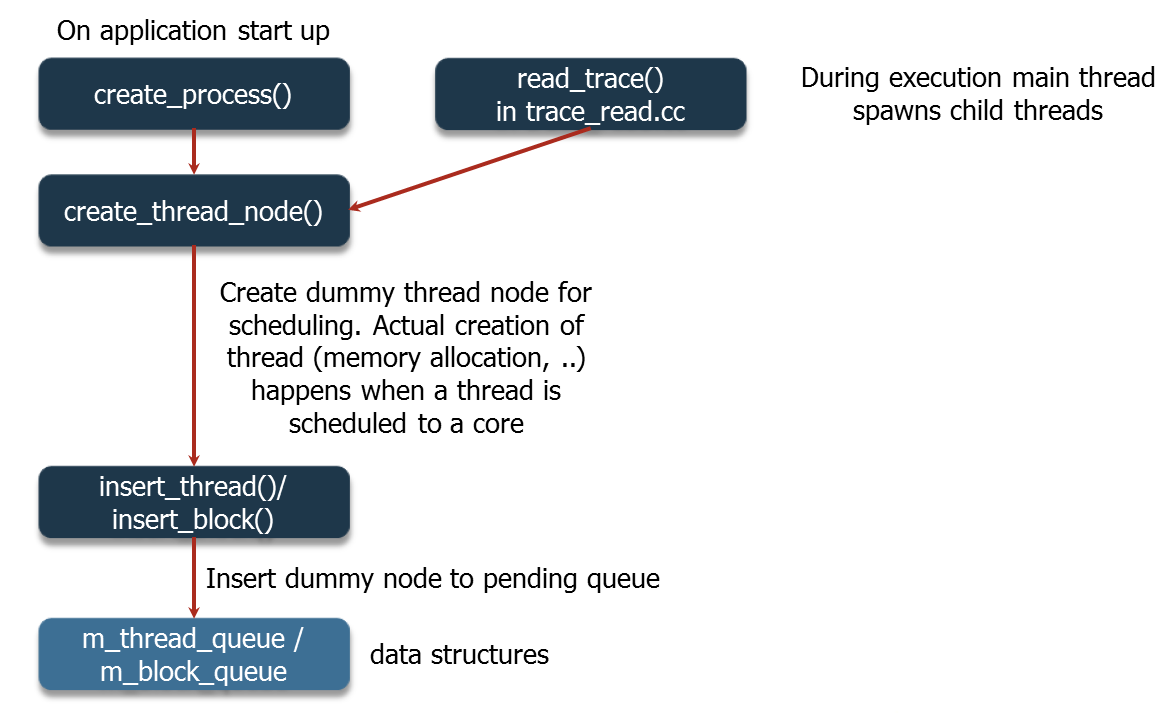
\includegraphics[height=80mm]{figs/process_creation}
\caption{Process and Thread Creation}
\label{fig:process_creation}
\end{figure*}

Figure~\ref{fig:process_creation} shows the control flow in the Process Manager on
simulation start up and during simulation. \textit{create\_process()} is called
for each application to be simulated. \textit{create\_process()} calls
\textit{setup\_process()} which in turn calls \textit{create\_thread\_node()}
for the main thread of the application. \textit{create\_thread\_node()}
allocates a \textit{thread\_trace\_info\_node\_s} instance for the main thread
and inserts it into \textit{m\_thread\_queue}. During the simulation of the
main thread when it is detected in \textit{read\_trace()} that a child thread
should be spawned, \textit{create\_thread\_node()} for the child thread is
called. The flow is similar for GPU kernels except that warps are inserted into
\textit{m\_block\_queue} instead of \textit{m\_thread\_queue}. Also, since GPU
kernels do not have a main thread, on kernel start up,
\textit{create\_thread\_node()} is called for the first warp in the
kernel. 

\begin{figure*}[htb]
\centering
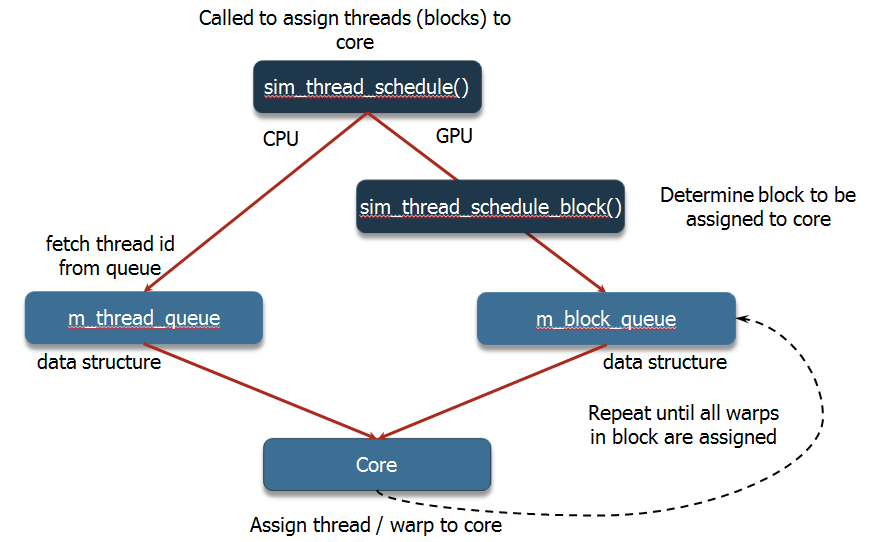
\includegraphics[height=80mm]{figs/thread_scheduling}
\caption{Thread/Thread Block Scheduling}
\label{fig:thread_scheduling}
\end{figure*}

When a thread/warp running on a core terminates,
\textit{sim\_thread\_schedule()} is called to schedule new threads/thread
blocks onto the core. Note that a new thread block can be assigned to a
core only when all warps of a previously assigned block have terminated.
\textit{sim\_thread\_schedule()} removes threads/warps from
\textit{m\_thread\_queue/m\_block\_queue} and assigns them to the core.
This flow is shown in Figure~\ref{fig:thread_scheduling}.

